\documentclass[12pt]{article}
\usepackage{amsmath,amsfonts,amsthm}
\usepackage{enumerate}
\usepackage{graphicx}
\usepackage{float}
\usepackage{multirow}
\usepackage{booktabs}
\usepackage{placeins}

\renewcommand{\baselinestretch}{1}
\topmargin 0in \headheight 0.0in \textheight 9in \textwidth 6.5in
\oddsidemargin 0.1in \evensidemargin 0.1in

\graphicspath{{../results/figures}}



\begin{document}

\title{Evaluating LASSO Performance in High-Dimensional Data: A Comparison Between Pixel and Frequency Domains}
\author{Siyang Ren, Nichole E. Carlson, William Lippitt, Yue Wang}
\date{}
\maketitle


\section*{Notes}

Everything surrounded by [] are my thoughts/questions/to-dos.


\section*{Introduction}

This study evaluates the performance of LASSO models in high-dimensional feature selection by comparing results from two different data representations: the original pixel space and a frequency space derived from eigen decomposition using Moran’s eigenvectors. The pixel space corresponds to the raw data where each feature is a pixel, while the frequency space transforms these features into frequency components.

We investigate whether fitting LASSO in the frequency space improves feature selection and prediction accuracy compared to the pixel space. Two simulation scenarios are used: one assuming sparsity in the pixel space and the other assuming sparsity in the frequency space. By comparing the results, we aim to determine which representation provides better performance for LASSO in high-dimensional datasets.


\section*{Methods}

Suppose \( \mathbf{x}=\left(x_1, \ldots, x_p\right)^T \) is a \( p \)-dimensional random vector. Its covariance matrix, \( \operatorname{var} (\mathbf{x}) = \boldsymbol{\Sigma} \), is a  \( p \times p \) matrix.

Whitening is a linear transformation that converts \( \mathbf{x} \) into a new random vector \( \mathbf{z}=\left(z_1, \ldots, z_p\right)^T \), using the transformation:
\[
  \mathbf{z}=\mathbf{W} \mathbf{x}
\]
where \( \mathbf{W} \) is a whitening matrix. The goal of whitening is to ensure that the covirance matrix of \( \mathbf{z} \) is the identity matrix \( \mathbf{I} \), meaning that all components of \( \mathbf{z} \) are uncorrelated and have unit variance:
\[
  \operatorname{var}(\mathbf{z})=\mathbf{I}
\]

We will show that in order for \( \mathbf{W} \) to be a valid whitening matrix, it must satisfy the condition:
\[
  \mathbf{W}^T \mathbf{W}=\boldsymbol{\Sigma}^{-1}
\]

\begin{proof}
  Let \( \mathbf{z} = \mathbf{W} \mathbf{x} \). The covariance of \( \mathbf{z} \) is:
  \[
    \operatorname{cov}(\mathbf{z}) = \mathbf{W} \operatorname{cov}(\mathbf{x}) \mathbf{W}^T = \mathbf{W} \boldsymbol{\Sigma} \mathbf{W}^T
  \]
  Since whitening ensures \( \operatorname{cov}(\mathbf{z}) = \mathbf{I} \), we have:
  \[
    \mathbf{W} \boldsymbol{\Sigma} \mathbf{W}^T = \mathbf{I}
  \]
  Multiplying both sides by \( \mathbf{W} \) gives:
  \[
    \boldsymbol{\Sigma} (\mathbf{W}^T \mathbf{W}) = \mathbf{I}
  \]
  Thus, \( \mathbf{W}^T \mathbf{W} = \boldsymbol{\Sigma}^{-1} \), as required.
\end{proof}

However, this constraint does not uniquely determine the whitening matrix \( \mathbf{W} \) \cite{Kessy_Lewin_Strimmer_2018}.

Whitening is useful because it ensures uncorrelation among variables, a desirable property in many analyses. A common choice of \( \mathbf{W} \) is
\[
  \mathbf{W}=\boldsymbol{\Lambda}^{-1 / 2} \mathbf{U}^T
\]
where \( \boldsymbol{\Sigma}=\mathbf{U} \boldsymbol{\Lambda} \mathbf{U}^T \) is the eigen-decomposition of the covariance matrix. 

\begin{proof}
  \[
    \mathbf{W}^T \mathbf{W}=\mathbf{U} \boldsymbol{\Lambda}^{-1 / 2} \boldsymbol{\Lambda}^{-1 / 2} \mathbf{U}^T=\mathbf{U} \boldsymbol{\Lambda}^{-1} \mathbf{U}^T
  \]
  Since \( \boldsymbol{\Sigma} \) is a covariance matrix, it is symmetric, which implies that \( \mathbf{U} \) is orthogonal, meaning \( \mathbf{U U}^T = \mathbf{I} \), so \( \mathbf{U}^T = \mathbf{U}^{-1} \). Therefore,
  \[
    \begin{aligned}
      \mathbf{U} \boldsymbol{\Lambda}^{-1} \mathbf{U}^T & = \left(\mathbf{U}^T\right)^{-1} \boldsymbol{\Lambda} \mathbf{U}^{-1} \\
                                                        & = \left(\mathbf{U} \boldsymbol{\Lambda} \mathbf{U}^T\right)^{-1} \\
                                                        & = \boldsymbol{\Sigma}^{-1}
  \end{aligned}
  \]
\end{proof}

Actually, a whitening matrix is not necessary to achieve uncorrelation. For example, using \( W^{\prime} = U^T \) from the eigen-decomposition is sufficient for this purpose.

\begin{proof}
  \[
    \operatorname{cov}\left(\mathbf{W}^{\prime} \mathbf{x}\right)=\mathbf{W}^{\prime} \boldsymbol{\Sigma} \mathbf{W}^{\prime T}=\mathbf{U}^T \boldsymbol{\Sigma} \mathbf{U}=\mathbf{U}^T \mathbf{U} \boldsymbol{\Lambda} \mathbf{U}^T \mathbf{U}=\boldsymbol{\Lambda}
  \]
  (since \( \mathbf{U}^T \mathbf{U}=\mathbf{I} \))
\end{proof}

Here, \( \Lambda \) is a diagonal matrix with eigenvalues on the diagonal. Therefore, we have shown that using the eigenvectors of a random vector's covariance matrix to perform a linear transformation resolves the correlation between the components, although it does not standardize their variance.

The Moran Coefficient (MC) is the most commonly used measure of spatial autocorrelation. Given a spatial pattern (e.g., an image with \( n \) pixels) represented as a vector \( \mathbf{y}=\left(y_1, \ldots, y_n\right)^T \), the Moran Coefficient \( \text{MC} (\mathbf{y}) \) is a value that indicates the strength of a spatial correlation. Larger absolute value represent strong spatial patterns, while values close to 0 indicate randomness. The expression for \( \text{MC} (\mathbf{y}) \) is written as \cite{Griffith_Chun_2014}:
\[
  M C(\mathbf{y})=\frac{n}{\sum_{i=1}^n \sum_{j=1}^n c_{i j}} \frac{\sum_{i=1}^n\left(y_i-\bar{y}\right)\left[\sum_{j=1}^n c_{i j}\left(y_j-\bar{y}\right)\right]}{\sum_{i=1}^n\left(y_i-\bar{y}\right)^2}
\]
where \( c_{ij} \) represents the spatial closeness between items \( i \) and \( j \). In matrix notation, this can be expressed as:
\[
  M C(\mathbf{y})=\frac{n}{1^{\prime} \mathbf{C} 1} \frac{\mathbf{y}^{\prime} \mathbf{M C M y}}{\mathbf{y}^{\prime} \mathbf{My}}
\]
Here, \( \mathbf{M}=\mathbf{I}-11^{\prime} / n \) is the centering matrix, which centers the vector \( \mathbf{y} \) by subtracing the mean.

Spatial filtering (\cite{Tiefelsdorf_Griffith_2007}) is a method [briefly describe what it does]. Eigenvector Spatial Filtering (ESF) is a methodology that utilizes eigenvectors extracted from the spatial closeness matrix \( \mathbf{C} \) to remove spatial dependencies. 

The decomposition of the double-centered matrix \( \mathbf{M C M} \) can be written as:
\[
  \mathbf{M C M}=\mathbf{E} \boldsymbol{\Lambda} \mathbf{E}^{T}
\]
where \( \boldsymbol{\Lambda} \) is a diagonal matrix of eigenvalues (in descending order), and \( \mathbf{E} \) is the matrix of corresponding eigenvectors. The eigenvectors have the property that \( \mathbf{e}_i^T \mathbf{e}_j=0 \) for \( i \neq j \), and \( \mathbf{e}_i^T \mathbf{e}_i=1 \). In matrix form, this means \( \mathbf{E E}^T=\mathbf{I} \). Additionally, each eigenvector satisfies \( \mathbf{e}_i^T 1 = 0 \) [which I haven't verified it yet.] Another important property of \(\mathbf{M}\) is that it is idempotent, meaning \(\mathbf{M M}=\mathbf{M}\). The last fact we will prove is that: \( \mathbf{E}=\mathbf{M E} \).

\begin{proof}

  Since \(\mathbf{E}\) is the matrix of eigenvectors, we have:

  \[
    \mathbf{M C M E}=\mathbf{E} \boldsymbol{\Lambda}
  \]

  Multiplying both sides by \(\mathbf{M}\) gives:

  \[
    \mathbf{MMCME}=\mathbf{ME} \boldsymbol{\Lambda}
  \]

  Since \(\mathbf{M}\) is idempotent, this simplifies to:

  \[
    \mathbf{MCME}=\mathbf{ME} \Lambda
  \]

  Thus:

  \[
    \mathbf{E} \boldsymbol{\Lambda}=\mathbf{M E} \boldsymbol{\Lambda}
  \]

  Cancelling \(\boldsymbol{\Lambda}\) (which is nonzero) from both sides gives:

  \[
    \mathbf{E}=\mathbf{M E}
  \]

\end{proof}

The Moran Coefficient for each eigenvector \(\mathbf{e}_i\) is proportional to its corresponding eigenvalue \(\lambda_i\). That is:

\[
  M C\left(\mathbf{e}_i\right)=\frac{n}{1^T \mathbf{C} 1} \lambda_i
\]

\begin{proof}

  \[
    M C\left(\mathbf{e}_i\right)=\frac{n}{\mathbf{1}^{\prime} \mathbf{C} \mathbf{1}} \frac{\mathbf{e}_i^{\prime} \mathbf{M C M e}_i}{\mathbf{e}_i^{\prime} \mathbf{M e}_i}
  \]

  Substituting \(\mathbf{M C M e}_i=\lambda_i \mathbf{e}_i\), we get:

  \[
    =\frac{n}{1^{\prime} \mathbf{C} 1} \frac{\mathbf{e}_i^{\prime} \mathbf{e}_i \lambda_i}{\mathbf{e}_i^{\prime} \mathbf{M e}_i}
  \]

  Since \(\mathbf{e}_i^{\prime} \mathbf{e}_i=1\) and \(\mathbf{M e}_i=\mathbf{e}_i\), this simplifies to:

  \[
    =\frac{n}{1^{\prime} \mathrm{C} 1} \lambda_i
  \]
\end{proof}



\subsection*{Data Simulation}

Let \( \mathbf{x} \) be a column vector representing the pixel values of a single observation, where the total number of pixels is \( n = 256 \). The covariance matrix \( \mathbf{C} \) follows an exponential correlation structure:
\[
\mathbf{C}_{ij} = -\exp(\operatorname{dist}(i,j)),
\]
where \( \operatorname{dist}(i,j) \) is the distance between pixels \( i \) and \( j \) on a \( 16 \times 16 \) grid. To center the data, we use the centering matrix \( \mathbf{M} = \mathbf{I} - \mathbf{1} \mathbf{1}^{\prime} / n \). The decomposition of \( \mathbf{MCM} \) is given by:
\[
\mathbf{MCM} = \mathbf{E}_{\text{full}} \mathbf{\Lambda}_{\text{full}} \mathbf{E}_{\text{full}}^{\prime},
\]
where \( \mathbf{E}_{\text{full}} \) represents the eigenvectors, and \( \mathbf{\Lambda}_{\text{full}} \) the diagonal matrix of eigenvalues \cite{murakami_eigenvector_2019}. The transformation of the pixel values \( \mathbf{x} \) into the frequency space is then:
\[
\mathbf{x}_{\text{freq}} = \mathbf{E}^T \mathbf{x}.
\]
Here, the covariance matrix of \( \mathbf{x}_{\text{freq}} \), \( \mathbf{E}^T \mathbf{C} \mathbf{E} \), is expected to be diagonal [this requires verification of \( \mathbf{E} \)'s orthogonality].

For each simulation, \( \mathbf{X} \) represents the matrix of observations, with each row corresponding to one of the 1000 total observations. The transformation of \( \mathbf{X} \) into the frequency domain is:
\[
\mathbf{X}_{\mathrm{freq}} = \mathbf{X} \mathbf{E}.
\]

We define the coefficient vectors in both spaces as follows: \( \boldsymbol{\beta} \) for the pixel space and \( \mathbf{b} \) for the frequency space. The relationship between the two is:
\[
\boldsymbol{\beta} = \mathbf{E} \mathbf{b},
\]
ensuring that \( \mathbf{X} \boldsymbol{\beta} = \mathbf{X}_{\mathrm{freq}} \mathbf{b} \).

Two simulation scenarios are considered:
\begin{enumerate}
  \item \textbf{Pixel space sparsity:} Here, \( \boldsymbol{\beta} \) is sparse, with non-zero values limited to a central \( 8 \times 8 \) region of the pixel grid. The covariate matrix \( \mathbf{X} \) is generated from a multivariate normal distribution with mean 0 and covariance matrix \( \mathbf{C} \). The response variable \( \mathbf{y} \) is binomial, with success probability determined by \( \boldsymbol{\eta} = \mathbf{X} \boldsymbol{\beta} \), where the non-zero entries in \( \boldsymbol{\beta} \) are constant and ensure that the success probability \( \mathbf{p} = \frac{1}{1 + \exp(-\boldsymbol{\eta})} \) is uniformly distributed in \( [0, 1] \).
  
  \item \textbf{Frequency space sparsity:} In this scenario, the coefficient vector \( \mathbf{b} \) is sparse, with 10\% of its 256 entries randomly set to non-zero values. The covariate matrix \( \mathbf{X}_{\mathrm{freq}} \) is generated from a multivariate normal distribution with zero mean and a diagonal covariance matrix, where the eigenvalues decrease along the diagonal [I am considering different options for the step size in the diagonal covariance matrix. Currently, I am using a constant step size, but further investigation may be needed to determine the most appropriate choice.]. The non-zero entries in \( \mathbf{b} \) are constant, and \( \mathbf{y} \) is drawn from a binomial distribution with a success probability \( \mathbf{p} \) uniformly distributed in \( [0, 1] \).

\end{enumerate}

After simulating data from either space, the values in the alternate space are calculated using the described transformations. When simulating data from the frequency space, even though the diagonal covariance matrix is chosen randomly and not calculated via \( \mathbf{E}^T \mathbf{C} \mathbf{E} \), \( \mathbf{E} \) is still used to transform the data back to the pixel space.

\subsection*{Model Evaluation}

To compare the performance of LASSO in both the pixel space and frequency space, we fit two models: one using covariates in the pixel space and another using covariates in the frequency space. The optimal regularization parameter \( \lambda \) is selected via cross-validation, using the binomial deviance as the performance metric. The dataset is split into training (80\%) and test (20\%) sets, and the cross-validation is performed using 10 folds.

Two values of \( \lambda \) are considered: 
\begin{itemize}
  \item \texttt{lambda.min}, which minimizes the cross-validated error.
  \item \texttt{lambda.1se}, the largest \( \lambda \) within one standard error of the minimum.
\end{itemize}

After selecting the optimal \( \lambda \), we evaluate model performance on the test set. The performance metrics include:
\begin{itemize}
  \item Accuracy
  \item Area Under the Curve (AUC)
  \item P-values for each covariate
\end{itemize}

P-values are computed using the \texttt{hdi} package [need to provide further details on how the package computes p-values]. The entire simulation is repeated 500 times. We report the mean and standard deviation of accuracy and AUC. For p-values, we report the percentage of cases where \( p < 0.05 \) at each covariate location [consider whether p-value adjustment is needed here].


\section*{Results}

\subsection*{Effect Size Determination}

In Simulation 1, we evaluated the distribution of the success probability \( \mathbf{p} \) at different non-zero values of \( \boldsymbol{\beta} \) (0.01, 0.05, 0.1, 0.2, and 1). As shown in Figure \ref{fig:sim1_p_dist}, a value of 0.1 produced the most uniform distribution of \( \mathbf{p} \), making it the optimal choice for model fitting in this scenario.

Similarly, in Simulation 2, we assessed the distribution of \( \mathbf{p} \) at various non-zero values for \( \mathbf{b} \) (0.1, 0.15, 0.2, 0.25, and 0.3). As shown in Figure \ref{fig:sim2_p_dist}, the value of 0.2 resulted in the most uniform distribution of \( \mathbf{p} \), making it the best option for this simulation.

\begin{figure}[h!]
	\centering
	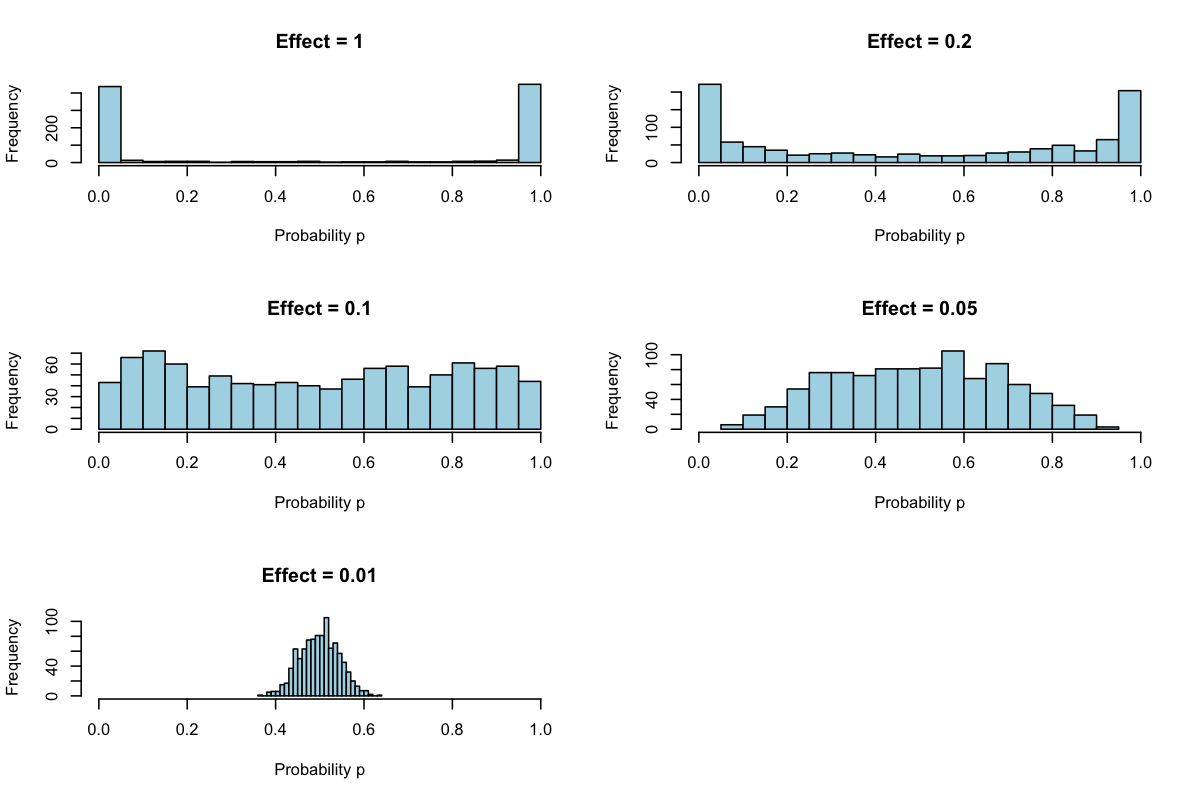
\includegraphics[width=0.8\textwidth]{sim1_p_dist.png}
  \caption{Distribution of success probability \( \mathbf{p} \) at different non-zero values in Simulation 1.}
	\label{fig:sim1_p_dist}
\end{figure}

\begin{figure}[h!]
	\centering
	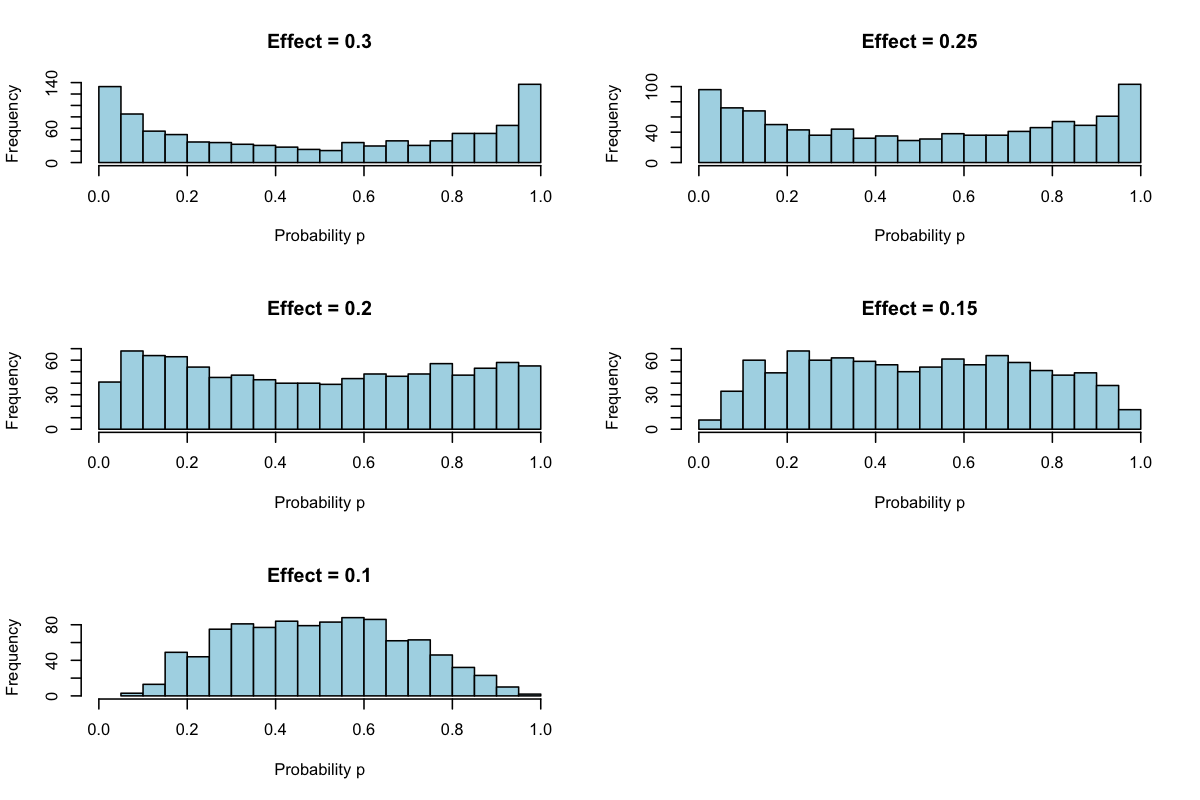
\includegraphics[width=0.8\textwidth]{sim2_p_dist.png}
  \caption{Distribution of success probability \( \mathbf{p} \) at different non-zero values in Simulation 2.}
	\label{fig:sim2_p_dist}
\end{figure}

\FloatBarrier

\subsection*{Group Mean Difference}

In this subsection, we examine the group mean differences in covariate values between instances where \( y = 1 \) and \( y = 0 \) for both Simulation 1 and Simulation 2.

Figure \ref{fig:group_diff1} presents the group mean differences for Simulation 1, with the heatmap on the left showing that regions corresponding to non-zero coefficients in \( \boldsymbol{\beta} \) exhibit larger mean differences between \( y = 1 \) and \( y = 0 \), as larger covariate values in these locations have higher probabilities of being assigned to \( y = 1 \). The scatterplot on the right displays the group mean differences in the frequency domain, where each point represents a frequency component; frequencies associated with larger eigenvalues tend to have larger mean differences. Figure \ref{fig:coefs_sim1} shows the actual coefficients used in Simulation 1, where non-zero coefficients in \( \boldsymbol{\beta} \) are localized to specific pixels, corresponding to the areas with larger mean differences in the group comparison.

\begin{figure}[h!]
	\centering
  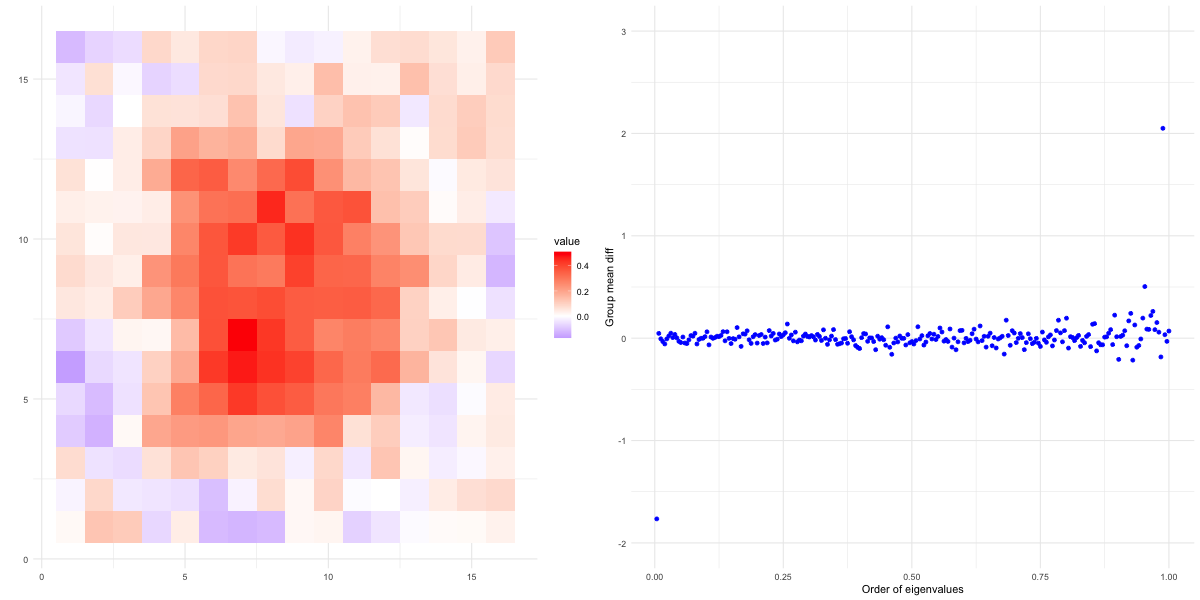
\includegraphics[width=0.8\textwidth, height=0.35\textwidth]{group_mean_diff_sim1.png}
	\caption{Group mean difference in covariate values between instances where \( y = 1 \) and \( y = 0 \) in Simulation
		1, shown for both the pixel space (left) and frequency space (right).}
	\label{fig:group_diff1}
\end{figure}

\begin{figure}[h!]
	\centering
	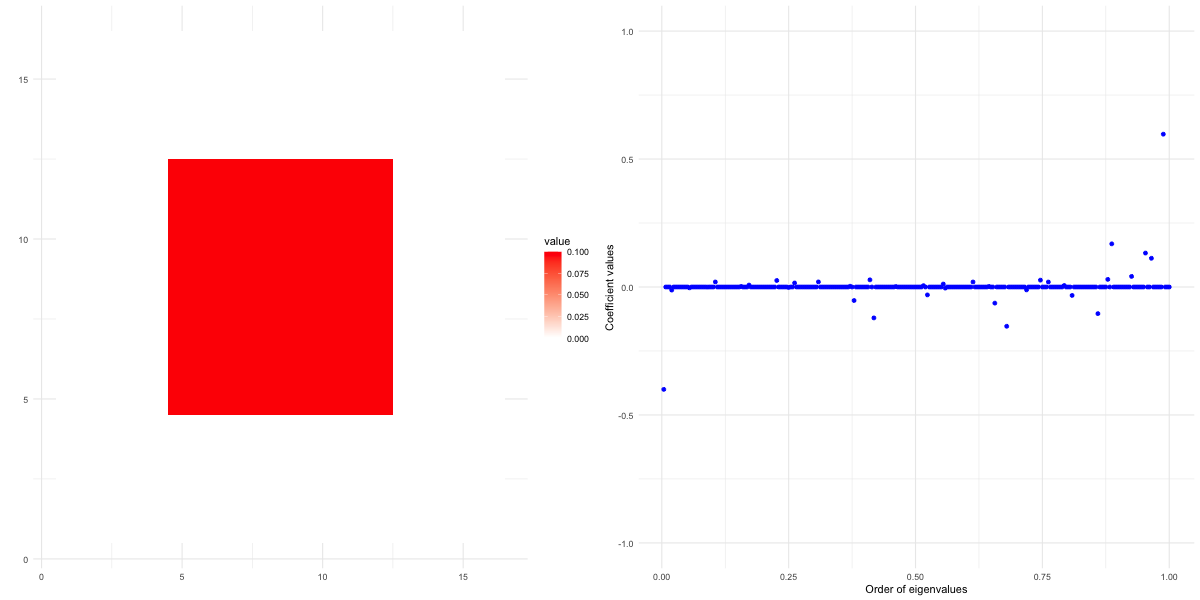
\includegraphics[width=0.8\textwidth, height=0.35\textwidth]{actual_coefs_sim1.png}
	\caption{Actual coefficients in Simulation 1 for the pixel space (left) and frequency space (right).}
	\label{fig:coefs_sim1}
\end{figure}

Figure \ref{fig:group_diff2} shows the group mean differences for Simulation 2, while Figure \ref{fig:coefs_sim2} displays the actual coefficients. The non-zero coefficients in \( \mathbf{b} \) are uniformly set to 0.2. However, the scatterplot in the frequency space does not clearly highlight the non-zero components, with increasing variance observed for larger eigenvalues. This variance pattern is consistent with the diagonal covariance matrix used in the simulation. The difficulty in identifying the non-zero components suggests that the effect size may be too small relative to the variance, making detection challenging. [Further adjustments to either the effect size or the covariance matrix could improve the detectability of these non-zero coefficients in future analyses.]

\begin{figure}[h!]
	\centering
	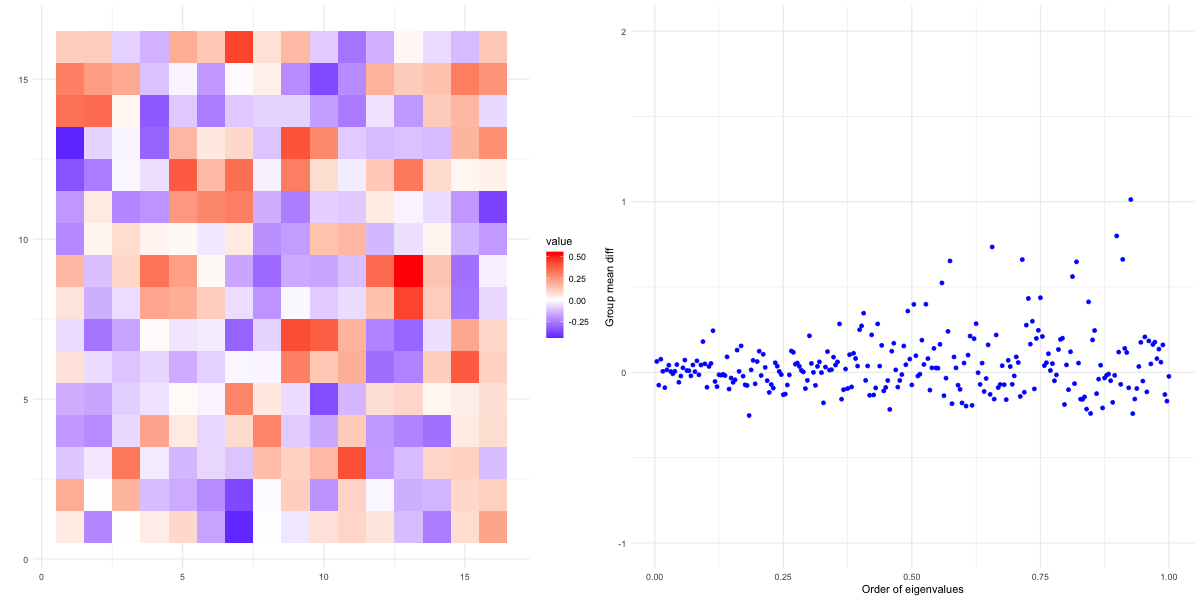
\includegraphics[width=0.8\textwidth, height=0.35\textwidth]{group_mean_diff_sim2.png}
	\caption{Group mean difference in covariate values between instances where \( y = 1 \) and \( y = 0 \) in Simulation 2.}
	\label{fig:group_diff2}
\end{figure}

\begin{figure}[h!]
	\centering
	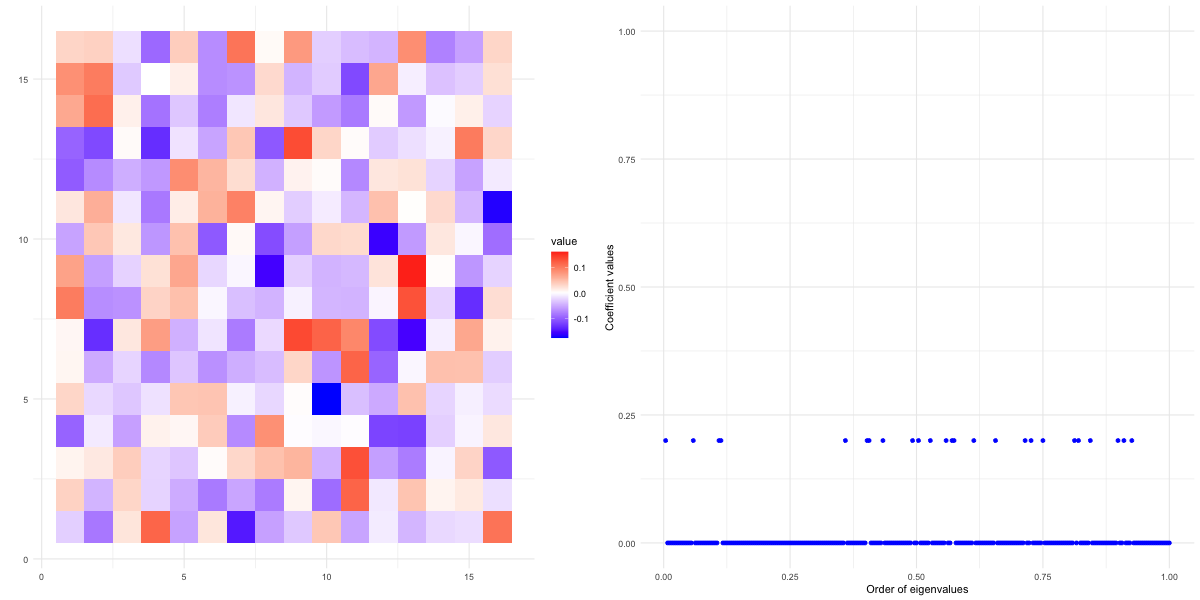
\includegraphics[width=0.8\textwidth, height=0.35\textwidth]{actual_coefs_sim2.png}
	\caption{Actual coefficients in Simulation 2 for the pixel space (left) and frequency space (right).}
	\label{fig:coefs_sim2}
\end{figure}

\FloatBarrier

\subsection*{AUC and Accuracy}

Table~\ref*{tab:auc_acc_table} summarizes the average AUCs and accuracies over 500 iterations. In both Simulation 1 (pixel space sparsity) and Simulation 2 (frequency space sparsity), models fitted in the frequency space consistently outperformed those fitted in the pixel space. For example, in Simulation 1, using \texttt{lambda.min} as the regularization parameter, models trained with pixel space covariates achieved an AUC of 0.803 (SE = 0.031) and an accuracy of 72.6\% (SE = 0.032). In contrast, models trained with frequency space covariates produced a slightly higher AUC of 0.826 (SE = 0.028) and a higher accuracy of 74.5\% (SE = 0.030). A similar trend was observed in Simulation 2, with frequency space models showing superior performance regardless of the regularization parameter used.

\begin{table}[h!]
	\centering
	\caption{Comparison of AUC and accuracy between models fitted in the pixel space and frequency space across 500 iterations for Simulation 1 and Simulation 2.}
	\label{tab:auc_acc_table}
	\begin{tabular}{l|cc|cc}
		\toprule
		\textbf{Simulation}   & \multicolumn{2}{c}{\textbf{Model in Pixel Space}} & \multicolumn{2}{c}{\textbf{Model in Frequency Space}}                                              \\
		\midrule
		                      & \textbf{AUC (SE)}                                 & \textbf{Accuracy (SE)}                                & \textbf{AUC (SE)} & \textbf{Accuracy (SE)} \\
		\midrule
		\textbf{Simulation 1} &                                                   &                                                       &                   &                        \\
    \texttt{lambda.min}            & 0.803 (0.031)                                     & 0.726 (0.032)                                         & 0.826 (0.028)     & 0.745 (0.030)          \\
      \texttt{lambda.1se}            & 0.800 (0.032)                                     & 0.722 (0.032)                                         & 0.826 (0.029)     & 0.745 (0.031)          \\
		\midrule
		\textbf{Simulation 2} &                                                   &                                                       &                   &                        \\
    \texttt{lambda.min}            & 0.755 (0.036)                                     & 0.684 (0.034)                                         & 0.812 (0.030)     & 0.732 (0.032)          \\
      \texttt{lambda.1se}            & 0.735 (0.039)                                     & 0.669 (0.038)                                         & 0.812 (0.031)     & 0.732 (0.032)          \\
		\bottomrule
	\end{tabular}
\end{table}

\subsection*{Coefficients Estimation}

Figure \ref{fig:b_estimates} presents the mean estimated \( b \) values plotted against the order of eigenvalues. The order of eigenvalues are calculated the same way as above. For Simulation 1, \texttt{lambda.1se} shrinks the estimated coefficients more than \texttt{lambda.min}, as it provides a larger panelty on it. For Simulation 2, even though it is not obvious, I feel the estimated values has an increase trend as the eigenvalues increase. [Still, I am wondering whether this is related to the covariance matrix, the decreased diagonal values, consider math proof?].

The mean estimated coefficients across iterations were calculated, and Figure \ref{fig:beta_estimates} displays the mean estimated \( \boldsymbol{\beta} \) values. Two key observations can be made: (1) There is no significant difference in the estimated coefficients when using \texttt{lambda.min} versus \texttt{lambda.1se}, and (2) the estimated values align well with the actual values, indicating that the model is accurately identifying the relevant features.

Figure \ref{fig:b_estimates} shows the mean estimated \( \mathbf{b} \) values plotted against the order of eigenvalues. The eigenvalue ordering is consistent with earlier calculations. In Simulation 1, \texttt{lambda.1se} applies a stronger regularization penalty, shrinking the estimated coefficients more than \texttt{lambda.min}. For Simulation 2, although the trend is less clear, there seems to be an upward trend in the estimated values as the eigenvalues increase. This trend may be related to the structure of the covariance matrix, specifically its decreasing diagonal values [consider math proof?].

\begin{figure}[h!]
	\centering
	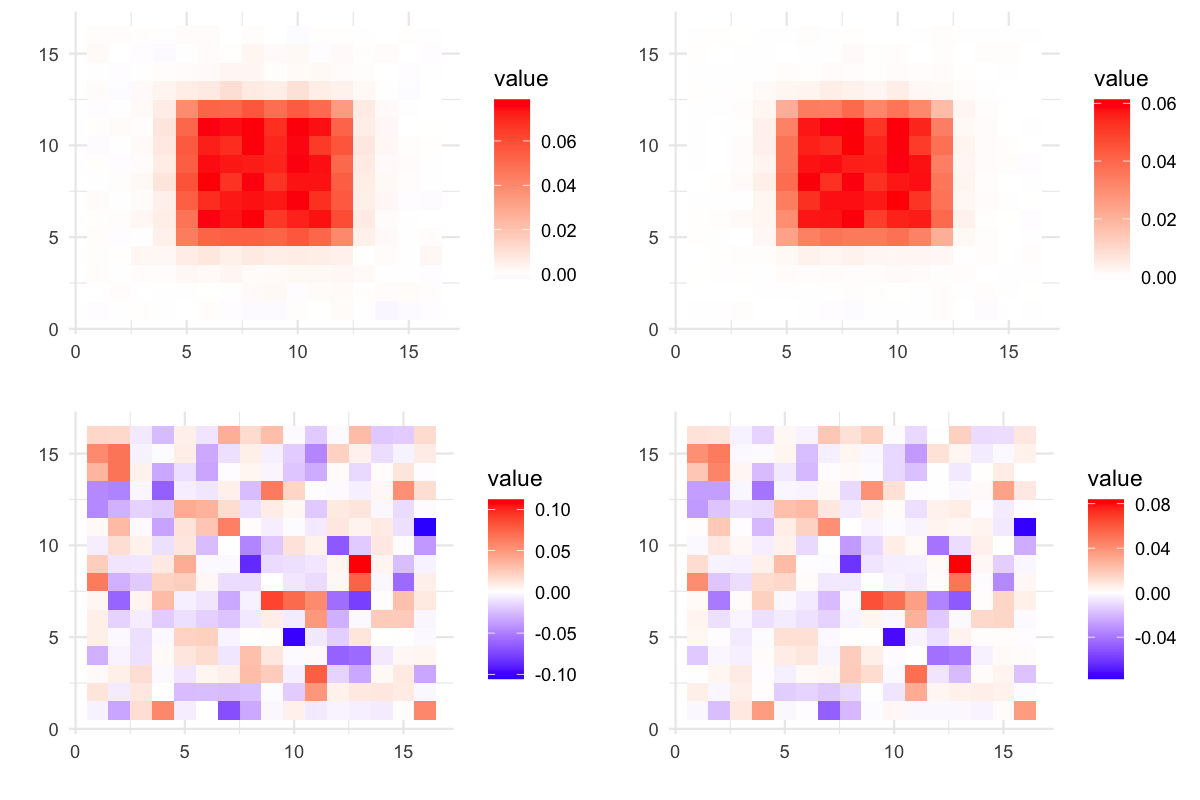
\includegraphics[width=0.8\textwidth]{beta_estimates.png}
	\caption{Mean estimated \( \beta \) values across simulations, with models fitted using \texttt{lambda.min} (left) and
		\texttt{lambda.1se} (right). The top row shows results for Simulation 1, while the bottom row shows results for Simulation 2.}
	\label{fig:beta_estimates}
\end{figure}

\begin{figure}[h!]
	\centering
	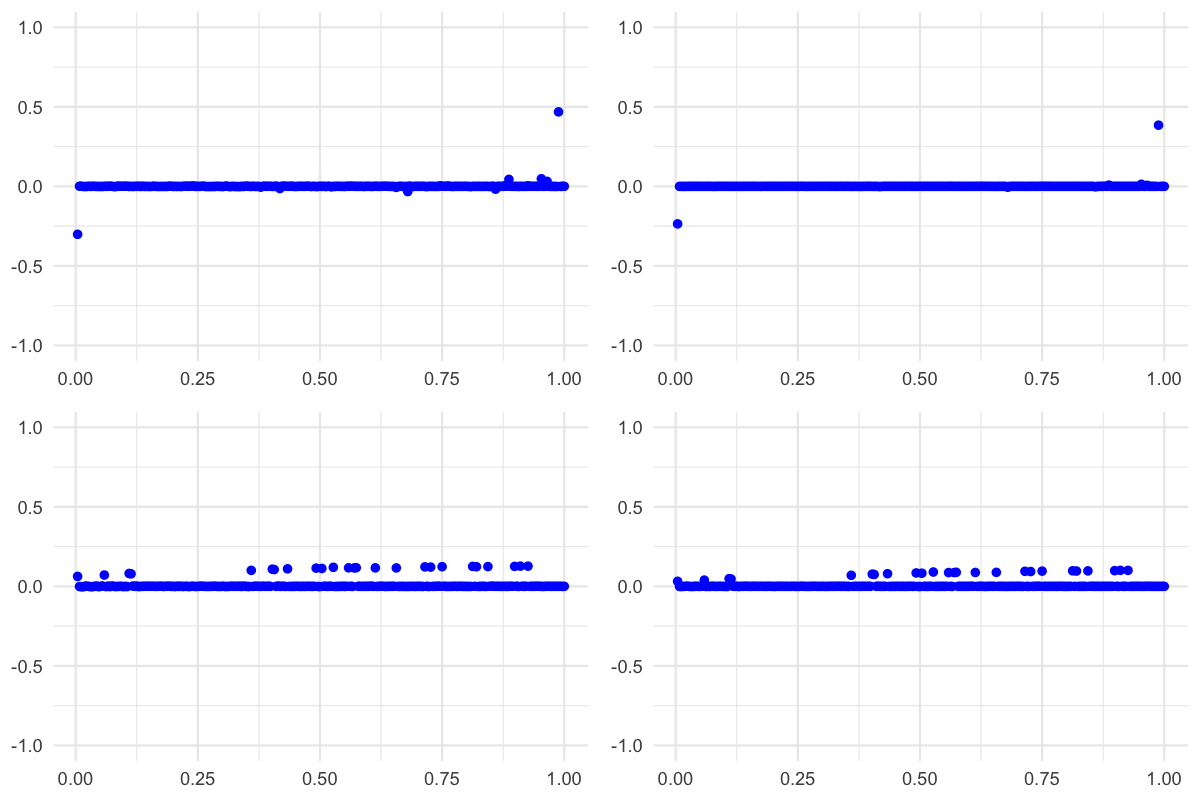
\includegraphics[width=0.8\textwidth]{b_estimates.png}
	\caption{Mean estimated \( b \) values across simulations, plotted against ordered eigenvalues. Models fitted using
		\texttt{lambda.min} are on the left and models fitted with \texttt{lambda.1se} on the right. The top row shows results for Simulation 1, while the bottom row shows results for Simulation 2.}
	\label{fig:b_estimates}
\end{figure}

\FloatBarrier

\subsection*{Significant P-values}

It is interesting to observe that, although the heatmap for significance of \( \boldsymbol{\beta} \) in Simulation 1 follows the pattern of the actual non-zero values, the percentage of significance is relatively low (Figure \ref{fig:perc_sign_beta} left). In contrast, the non-zero values of \( \mathbf{b} \) (Figure \ref{fig:perc_sign_b} left) show a much higher percentage of significance, reaching as high as 100\% across iterations.

Another observation is that, although the non-zero effect size for \( \mathbf{b} \) is constant in Simulation 2, the percentage of significant p-values increases as the eigenvalues grow (Figure \ref{fig:perc_sign_b} right). [I am considering creating a plot to visualize the actual \( \beta \) values in Simulation 2 and the actual \( b \) values in Simulation 1, where the non-zero values vary, and compare them with the corresponding percentage of significant p-values. The goal is to examine whether the size of the actual non-zero values correlates with the percentage of significance. I suspect that a larger absolute effect size should result in a higher percentage of significance, but this doesn’t seem to be the case for \( b \) in Simulation 2, so I want to investigate other factors as well.]

\begin{figure}[h!]
	\centering
	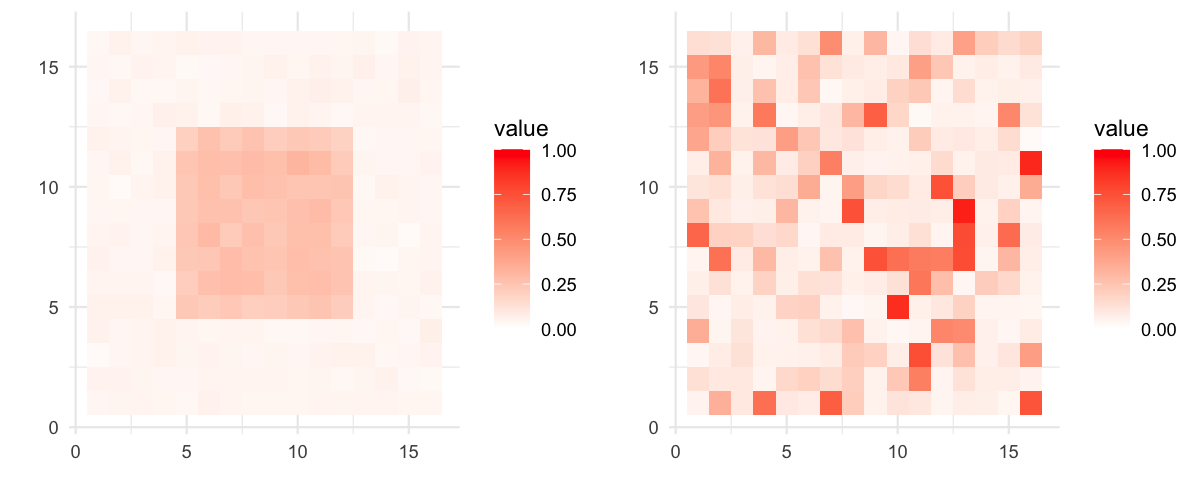
\includegraphics[width=0.9\textwidth]{perc_sign_pvals_hdi_beta.png}
	\caption{Percentage of significant p-values for elements of \( \beta \) when fitting models in the pixel space in
		Simulation 1 (left) and Simulation 2 (right).}
	\label{fig:perc_sign_beta}
\end{figure}

\begin{figure}[h!]
	\centering
	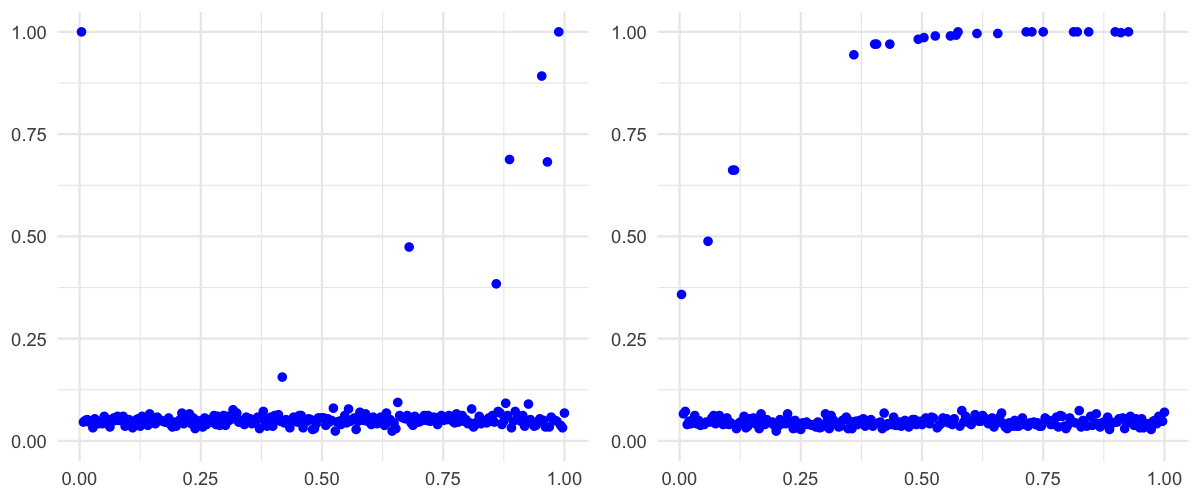
\includegraphics[width=0.9\textwidth]{perc_sign_pvals_hdi_b.png}
	\caption{Percentage of significant p-values for elements of \( b \) across ordered eigenvalues in both simulations.}
	\label{fig:perc_sign_b}
\end{figure}

\FloatBarrier


\section*{Future Work}

\begin{itemize}
  \item Adding details about how \texttt{hdi} package calculated p-values and why my permutation test didn't work.
  \item Increase \( b \) effect size (how to keep \( p \) evenly distributed in the same time?) see whether the pattern of coefficient estimates disappear or relieve.
  \item What is the next step in higher level?
\end{itemize}

\footnotesize
\bibliographystyle{abbrv}
\bibliography{references}

\end{document}


